%%%%%%%%%%%%%%%%%%%%%%%%%%%%%%%%%%%%%%%%%%%%%%%%%%%%%%%%%%%%%%%%%%%%%%%%
%    INSTITUTE OF PHYSICS PUBLISHING                                   %
%                                                                      %
%   `Preparing an article for publication in an Institute of Physics   %
%    Publishing journal using LaTeX'                                   %
%                                                                      %
%    LaTeX source code `ioplau2e.tex' used to generate `author         %
%    guidelines', the documentation explaining and demonstrating use   %
%    of the Institute of Physics Publishing LaTeX preprint files       %
%    `iopart.cls, iopart12.clo and iopart10.clo'.                      %
%                                                                      %
%    `ioplau2e.tex' itself uses LaTeX with `iopart.cls'                %
%                                                                      %
%%%%%%%%%%%%%%%%%%%%%%%%%%%%%%%%%%
%
%
% First we have a character check
%
% ! exclamation mark    " double quote  
% # hash                ` opening quote (grave)
% & ampersand           ' closing quote (acute)
% $ dollar              % percent       
% ( open parenthesis    ) close paren.  
% - hyphen              = equals sign
% | vertical bar        ~ tilde         
% @ at sign             _ underscore
% { open curly brace    } close curly   
% [ open square         ] close square bracket
% + plus sign           ; semi-colon    
% * asterisk            : colon
% < open angle bracket  > close angle   
% , comma               . full stop
% ? question mark       / forward slash 
% \ backslash           ^ circumflex
%
% ABCDEFGHIJKLMNOPQRSTUVWXYZ 
% abcdefghijklmnopqrstuvwxyz 
% 1234567890
%
%%%%%%%%%%%%%%%%%%%%%%%%%%%%%%%%%%%%%%%%%%%%%%%%%%%%%%%%%%%%%%%%%%%
%
%\documentclass[12pt]{iopart}
\documentclass[twocolumn,10pt]{asme2e}
%\newcommand{\gguide}{{\it Preparing graphics for IOP Publishing journals}}
%Uncomment next line if AMS fonts required
%\usepackage{iopams}  

\usepackage{epsfig} %% for loading postscript figures

	\expandafter\let\csname equation*\endcsname\relax		 %resolves conflict with amsmath package
	\expandafter\let\csname endequation*\endcsname\relax		 %resolves conflict with amsmath package
\usepackage{graphicx}
\usepackage{enumerate}
%\usepackage{subfigure}  %NOW DEPRICATED - 
\usepackage{wrapfig}
%SMS....%\usepackage{multicol}
\usepackage{booktabs}
\usepackage{multirow}
\usepackage{array}
\usepackage{amssymb,amsmath}
	\DeclareMathOperator{\sgn}{sgn}
\usepackage{epstopdf}
%\usepackage[compatibility=false]{caption}  %needed the compatibility = false command to deal with an error
\usepackage{subcaption}
%SMS....\usepackage[margin=1in]{geometry}
%SMS....\usepackage[margin=20pt,font=small,labelsep=endash]{caption}
\usepackage{url}

\confshortname{ASME SMASIS 2017}
\conffullname{the ASME 2017 Conference on Smart Materials, Adaptive Structures and Intelligent Systems}
%  \&\\
 %             Computers and Information in Engineering Conference}

%%%%% for date in a single month, use
\confdate{18-20}
\confmonth{September}
%%%%% for date across two months, use
%\confdate{August 30-September 2}
\confyear{2017}
\confcity{Snowbird, UT}
\confcountry{USA}

%%% Replace DETC2010/MECH-12345 with the number supplied to you 
%%% by ASME for your paper.
\papernum{SMASIS2017-3803}


\title{A novel biomimetic torsional actuator design using \\ twisted polymer actuators}

%%% first author
\author{Michael W. Shafer
    \affiliation{ 
	Assistant Professor\\
	Dept. of Mechanical Engineering\\
	Northern Arizona University\\
	Flagstaff, Arizona 86001\\
    Email: Michael.Shafer@nau.edu
    }
}

\author{Heidi P. Feigenbaum
    \affiliation{ 
	Associate Professor\\
	Dept. of Mechanical Engineering\\
	Northern Arizona University\\
	Flagstaff, Arizona 86001\\
    Email: Heidi.Feigenbaum@nau.edu
    }
}

\author{Diego Ricardo Higueras Ruiz 
    \affiliation{ 
	M.S. Candidate \\
	Dept. of Mechanical Engineering\\
	Northern Arizona University\\
	Flagstaff, Arizona 86001\\
      Email: DiegoRicardo@nau.edu
    }
}


\begin{document}

\maketitle    

\begin{abstract}

Artificial muscle systems have the potential to impact many technologies ranging from advanced prosthesis to miniature robotics. Recently, it has been shown that twisting drawn polymer monofilaments, such as nylon fishing line or sewing thread, can result in a biomimetic thermally activated torsional actuator. The actuation phenomenon in these twisted polymer actuators (TPAs) is thought to be a result of an untwisting that occurs about the fiber's axis due to an asymmetric thermal expansion. Before being twisted, the precursor fibers are comprised of polymer chains that are aligned axially. During fabrication of TPAs, the polymer chains reorient as the precursor fiber is twisted about the central axis of the monofilament. At the end of the fabrication process, the TPA is annealed in order to relieve internal stresses and to keep the fiber in the twisted configuration. The mechanism of  untwisting actuation is generally thought to be a result of radially expansion and axially contraction. After being twisted, these radial and axial expansion relationships remain relatively unchanged, but the polymer chain direction is no longer axially aligned. Thus, upon heating the twisted fibers of the TPA, the fibers untwist and torsional actuation occurs. This actuation phenomenon has been used in the past to create linear actuators, but cab also be use directly as a torsional actuator. Compared to other torsional actuators TPAs are low cost, lightweight, and can actuate reasonably high torques per unit volume.  However, because TPAs are thermally activated, they may not be suitable for all applications. In this work, we present a novel TPA design for use as a torsional actuator for miniature actuation and artificial muscle applications. Our design bundles twisted monofilaments to increase the torque. Both fabrication and testing methods of the new design are presented. Results for temperature versus torsional displacement under various loads give insights as to how these actuators may be used and the reversibility of the actuation process. Additionally, comparisons are made between these bundled actuators and similarly loaded single TPA monofilament actuation. 

%with heating wire to supply the temperature change and induce actuation. The conceptual design of this novel torsional actuator is presented here, along with the unloaded free rotation response of various configurations. Experimental characterization of the design includes direct temperature measurements of the TPA using an attached thermocouple, and  torsional displacement measured using video recordings of the actuation.  Results of these tests are presented and comparisons are made between the various configurations. Based on these results, we suggest further improvements that could be made to the design of these torsional actuators.  
\end{abstract}

% Uncomment for PACS numbers
%\pacs{00.00, 20.00, 42.10}
%
% Uncomment for keywords
%\vspace{2pc}
%\noindent{\it Keywords}: XXXXXX, YYYYYYYY, ZZZZZZZZZ
%
% Uncomment for Submitted to journal title message
%\submitto{\JPA}
%
% Uncomment if a separate title page is required
%\maketitle
% 
% For two-column output uncomment the next line and choose [10pt] rather than [12pt] in the \documentclass declaration
%\ioptwocol
%


\section{Introduction}
It was recently shown that drawn polymer monofilament such as nylon fishing line have the ability to act as linear actuators when twisted and configured helically if exposed to temperature changes \cite{haines_artificial}. The same monofilaments can be torsional actuators if twisted but not coiled helically \cite{haines_artificial, aziz_controlled}.  In the pursuit of an thermo-mechanical actuation model for these twisted polymer systems, our group has looked toward understanding how twisted polymer monofilaments would react torsionally when exposed to temperature changes \cite{shafer_first}. As part of this modeling effort, concepts in torsional actuation configurations were conceived. This work presents conceptual designs and actuation performance for a torsional actuator based on two configurations of a twisted polymer actuator (TPA). 

Twisted polymer actuators, when configured to act as a linear actuator, are often classified as a type of artificial muscle. A wide variety of artificial muscle technologies exist for linear actuation. While less work has focused on how smart materials can be configured for torsional actuation, there are still a number of materials in use. Some of these technologies use a linear actuation phenomenon in a helical configuration to induce a twisting. Nitinol shape memory alloys (SMA), typically used for linear actuation, have been used in a tube configuration to create a torsional actuator \cite{jardine_shape}. Many other torsional actuation technologies rely on  radial changes of materials in helical configurations. Electroactive polymers, pneumatic and hydraulic artificial muscles, and carbon nanotubes, have all been used in a helical configuration to create torsional actuation through radial changes \cite{suh_torsional,chun_hybrid,fang_fiber,sanan_pneumatic}. While the method of radial changes varies between materials, the mechanism of actuation remains the same and relies on increasing the path length for helically wrapped fibers. Each of these technologies has impressive performance in at least one metric, but none are as simple and inexpensive as torsional TPAs.

In discussing these polymer actuators, it is important to make clear the differences in terminology regarding `twist' and `coil'. A precursor fiber is considered to be a straight drawn polymer fiber, such as monofilament fishing line, while a twisted fiber is one in which a precursor fiber is twisted about its central axis but remains straight. Although a twisted precursor fiber will remain straight, after twisting its polymer chains will be helically oriented about the precursor fiber's axis with a pitch angle that depends on radial position. Figure \ref{fig:helix} highlights how twisting reorients the polymer chains into a helical configuration with a radially dependent pitch. Typically, after twisting the material is annealed so that internal stresses are relieved and the material remains twisted when unloaded. Coiling refers to a fiber, twisted or untwisted, that is annealed in a helical configuration. This helical configuration can be developed by increasing the amount of twist in a precursor fiber to a point at which the fiber torsionally buckles and coils over on itself, or helically wrapping the material on a mandrel. With these definitions for `twisting' and `coiling,' we use the terms `straight-twisted polymer actuators' (STPA) to refer to the torsional actuators that are not coiled, and `twisted-coiled polymer actuators' (TCPA) to refer the linear actuators in the helical configuration. 

Individual straight twisted polymer actuators can be used to generate low torque torsional actuations similar to the way in which CNT yarns have been used in the past \cite{suh_torsional}, but at significantly lower cost \cite{aziz_controlled}. In this work, we present isotonic torsional actuation performance for such a monofilament STPA configuration. We also consider here the configuration of STPAs wrapped into a parallel configuration such that multiple STPAs work together to generate a torque. This configuration can be seen in Figure \ref{fig:micro_para}. We use the term parallel configuration to indicate that the monofilaments actuate in parallel, not that they are parallel to the bungle's axis. Such a parallel configuration is fabricated using standard rope making manufacturing processes, and as such, allows for a wide variety of potential configurations of parallel STPA elements, structural elements, and heating elements. The isotonic concentric and eccentric actuation performance of these parallel STPA configurations are shown here. As part of this study, we present the fabrication techniques for monofilament STPAs and parallel STPAs. We also show how a core can be added to the parallel configuration in order to allow for direct heating of the actuator from within the actuator. The stroke-temperature relationship is investigated for both monofilament and parallel actuator designs for two different preload torques. We highlight a unique initial actuation cycle response that is observed which would need to be accounted for in practical applications of these actuators.
\begin{figure}
    \centering
     \begin{subfigure}[b]{0.5\textwidth}
        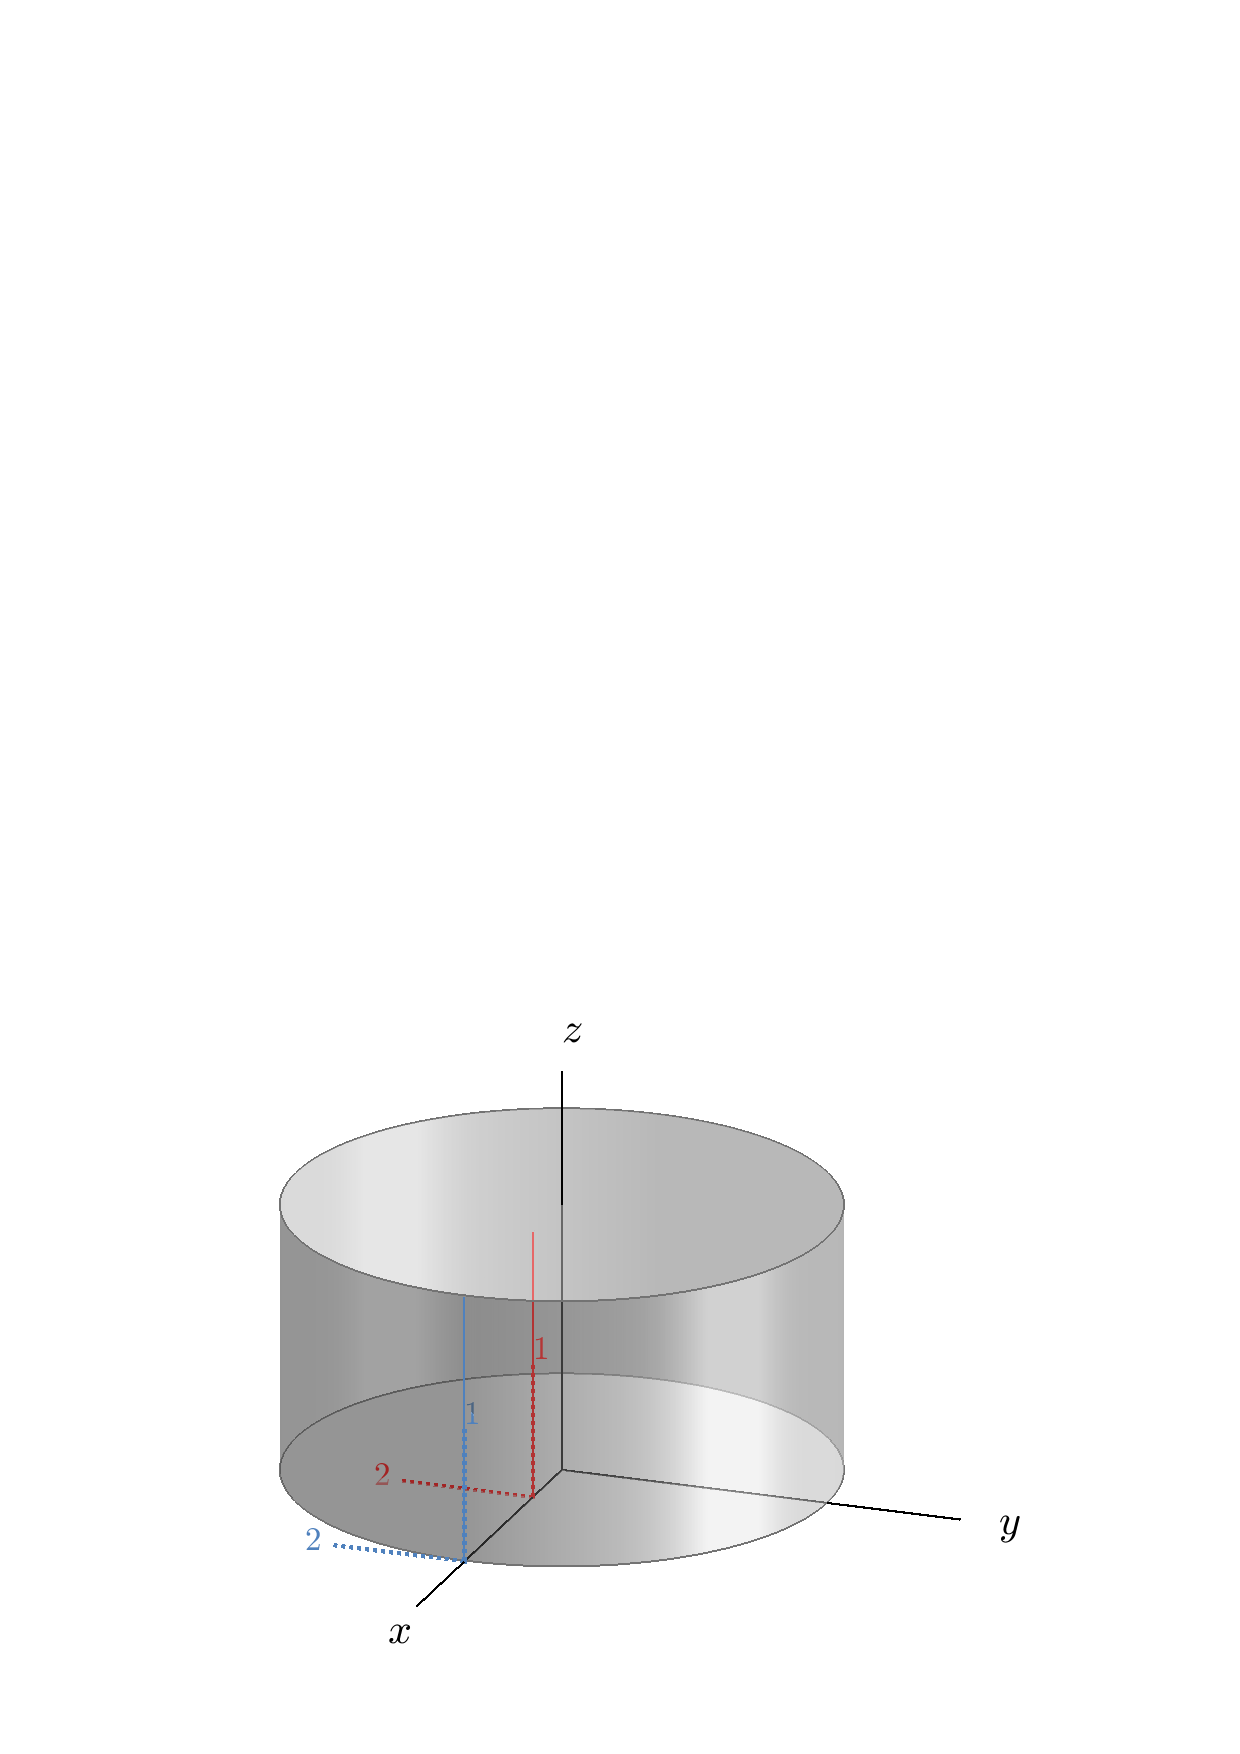
\includegraphics[width=7cm, clip = true, trim = {0.8in 0.5in  0.8in 0.8in}]{../Images/helix_2_initial.pdf}
        \caption{Initial configuration }
        \label{fig:helix_init}
        \end{subfigure}
     \begin{subfigure}[b]{0.5\textwidth}
        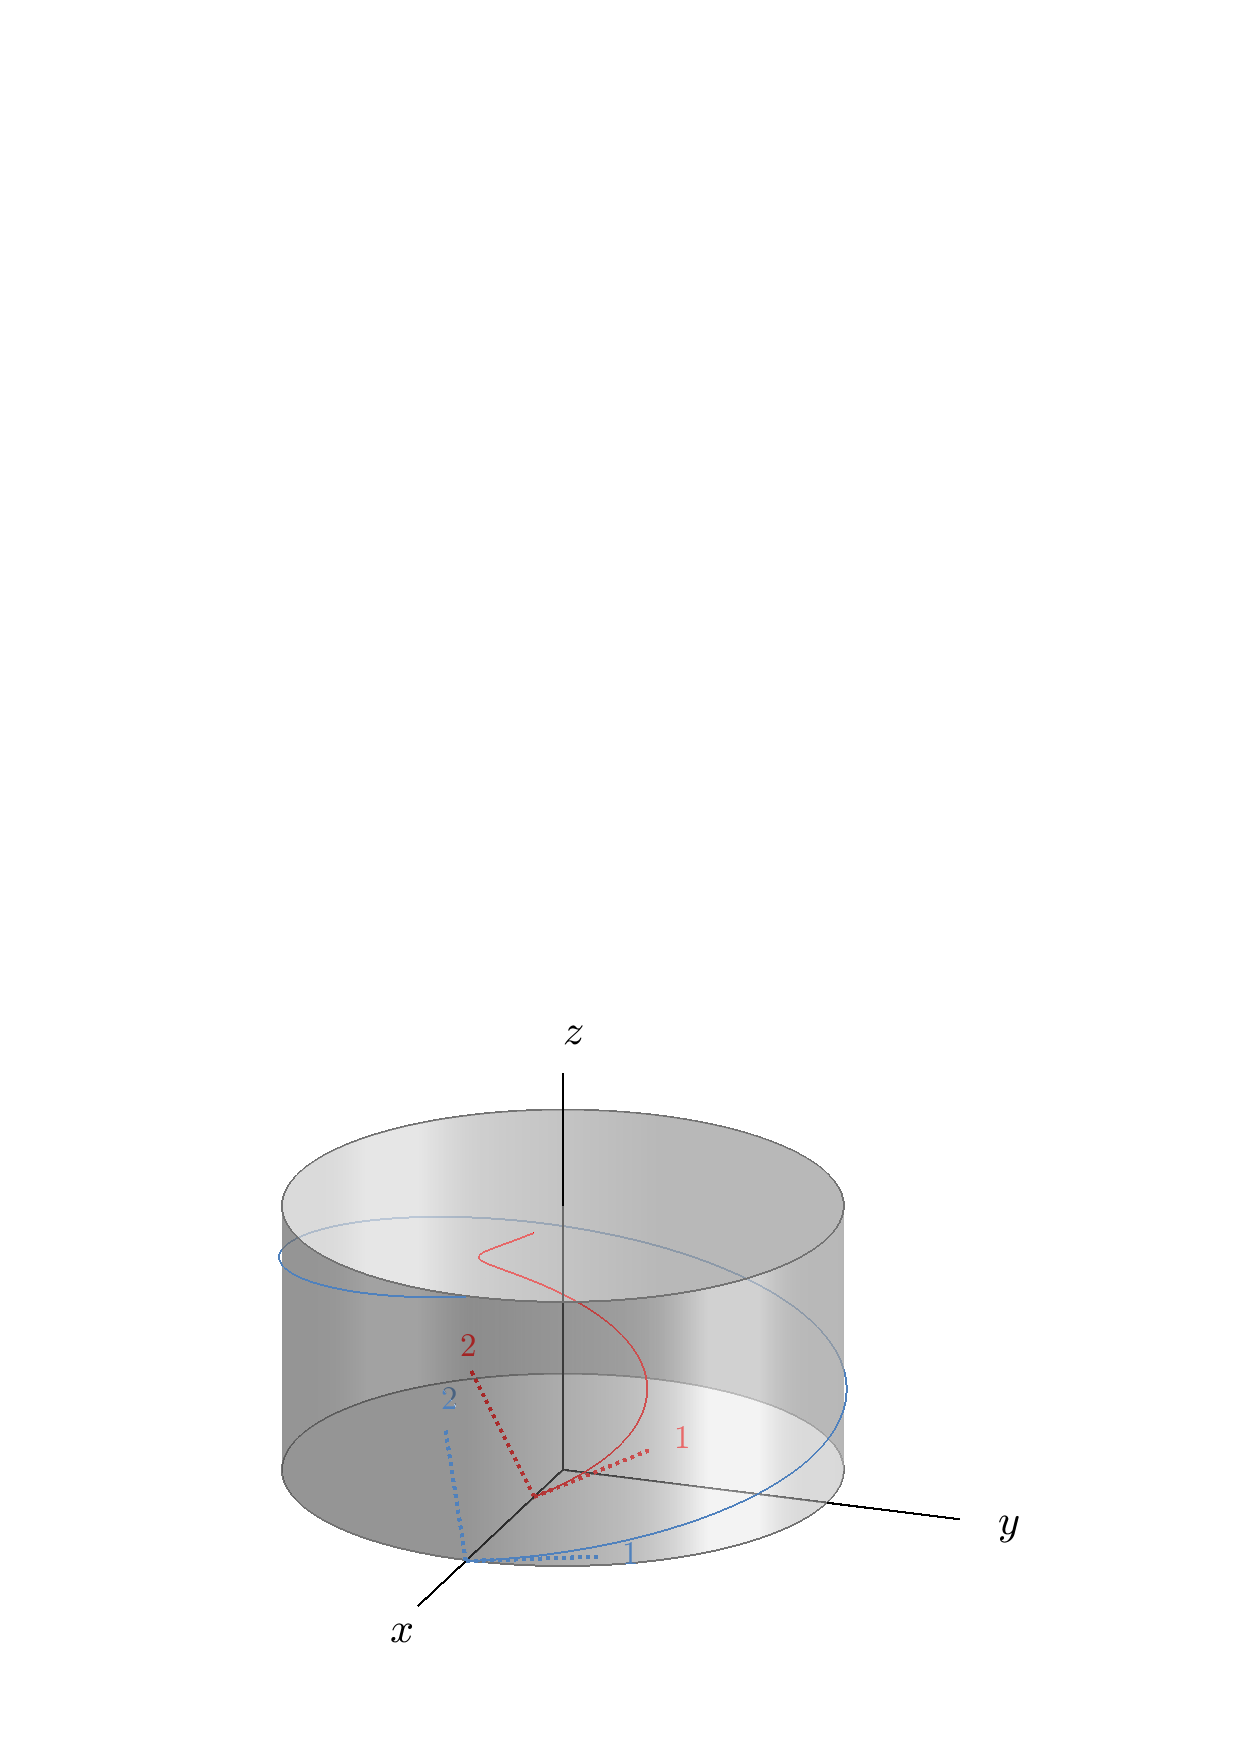
\includegraphics[width=7cm, clip = true, trim = {0.8in 0.5in  0.8in 0.8in}]{../Images/helix_2.pdf}
        \caption{Twisted and annealed configuration}
        \label{fig:helix_final}
        \end{subfigure}
        \caption{Conceptual diagram showing (\subref{fig:helix_init}) untwisted and (\subref{fig:helix_final}) twisted monofilament with lines representing polymer chain configurations. Notices that angle of polymer chain (1-direction) with respect to the $x-y$ plane ($\alpha$) depends on radial position after twisting.}
        \label{fig:helix}
\end{figure}

\section{Fabrication of torsional twisted polymer actuators}
The single monofilament STPA configuration presented in this work as a basis of comparison to the parallel configuration were manufactured in a way similar to previous works that have investigated torsional and linear actuation of TPAs. A straight precursor fiber was twisted under a small tensile force and held in this configuration during a subsequent annealing process. A monofilament STPA torsional actuator can be seen in Figure \ref{fig:micro_mono}. Specific pitch angle can are achieved by relating the number of twists inserted per unit length ($T$) to the diameter of the precursor fiber ($D$) through:
\begin{equation}
\alpha_f = \tan^{-1}{\pi D T}
\end{equation}
Rather than employing a single monofilament STPA torsional actuator, many can be wound together to crease a ``parallel'' configuration wherein multiple fibers are twisted together so that they act as torsional actuators in parallel. This configuration can be seen in figure \ref{fig:micro_para}. These configurations  are fabricated using a similar method as twisted rope. A simple triple twisted rope making machine is composed of a rigid tower, where three hooks are positioned at the vertices of an equilateral triangle. A diagram of the system used to make the actuators is shown in Figure \ref{fig:coiled}. A second movable tower is located at the opposite side of the device and includes a centrally located forth hook. We also include a central fifth hook at the center of the equilateral triangle on the primary support which allows for the inclusion of a structural or heater element core. 

During the fabrication of these parallel configuration STPA actuators, a NiCr heating wire was located in the core of the TPA coil by installing it between right side tower and the central hook on the left side tower of Figure \ref{fig:coiled}. During the coiling process, the three hooks were rotated clockwise, while the fourth and the fifth hook will be rotated counterclockwise. Thus the central heating wire was not be twisted but the precursor nylon monofilaments experienced a torsion. Due to this fact, the actuator shrinks during this fabrication process necessitating movement of the right side tower during twisting. The amount of tension maintained during this twisting is likely related to the final actuation perfomance. During the fabrication of the actuators tested for this work, only a minimal tension was maintained during coiling. 

After twisting these actuators, the twisting hooks were locked in place to prepared for the annealing process. The assembly with the mounted TPA was then placed in an oven at a temperature of 120$^\circ$C for 20 minutes. Subsequently, the assembly was removed from the oven and allowed to freely cool before the removal of the actuator from the fabrication rig. Finally, the sample was cut to length. For the samples tested in this work, the two ends of the cut same were fixed by with cyanoacrylate glue. 

\begin{figure}
    \centering
     \begin{subfigure}[b]{0.15\textwidth}
        \includegraphics[width=3.5cm]{../Images/micro_mono.pdf}
        \caption{}
        \label{fig:miro_mono}
        \end{subfigure}
        \quad \quad  \quad \quad
     \begin{subfigure}[b]{0.15\textwidth}
        \includegraphics[width=3.5cm]{../Images/micro_para.pdf}
        \caption{}
        \label{fig:micro_para}
        \end{subfigure}
        \caption{Microscope images showing (a) an monofilament STPA with pitch angle of $30^\circ$ and (b) a parallel STPA actuator with the same pitch angle as the monofilament configuration. Also visible in (b) is how a NiCr heater wire element can be spliced within the parallel STPA configuration.  }
        \label{fig:micro}
\end{figure}


\begin{figure}
    \centering
        \includegraphics[width=8cm]{../Images/coiling_rig.pdf}
        \caption{Fabrication rig for torsional TPA based on twisted rope fabrication process. During the twisting process the precursor fibers are twisted in a direction opposite to that of the hook on the right. If a central heating or structural core is use, the center hook on the left is turned at the same rate as that on the right to maintain zero twist in the core. }
        \label{fig:coiled}
\end{figure}

\section{Methods for isotonic torsional stroke testing}
In order to characterize these torsional actuators, an experimental setup was designed and built which maintained a constant torque on the actuators during heating. A preload torque is known to be required to bring these actuators back to their initial angle state after cooling. The experimental setup included a 3D printed frame, ball bearing, torque spool, clamp, and weight. This setup can be see in Figure \ref{fig:setup}. In this figure, the actuator sample can be seen to be clamped on the right of the frame. The left side of the sample is glued into the torque spool, a hollow pulley that interfaces with a bearing pair. A pair of ball bearings are used to react both the moment and radial loads passed into the torque spool from the weight. This weight hangs from the 6 mm diameter torque by a fine steel wire. 

The position of the weight is measured using a Polytec OVF-5000/OVF-534 vibrometer controller and sensor unit, along with DD-900 Digital Displacement Decoder unit. The voltage output of this system is linearly related to a change of position of the object on which it focuses. This voltage is recorded by a National Instruments PXI-6361 multifunction data acquisition card, which simultaneously samples temperature measurement from the K-type thermocouple embedded within the test sample as shown in figure \ref{fig:setup}. Ambient room temperature is noted from the sample temperature prior to the application of a thermal load. Temperature and displacement measurements are recorded at 100 Hz and then later smoothed using a moving average filter to a sampling frequency of 10Hz. For single monofilament tests wherein the thermocouple could not be embedded into the actuator, the thermocouple was taped to the surface of the sample. 

Each test was initiate by clamping an actuator sample in a frame and applying a preload torque by attaching a weight to the cable on the torque spool. The laser vibrometer zero position was then reset, and the data acquisition system was started. A hot air source was then placed adjacent to the sample to heat the actuator. When the temperature of the actuator reached between 90-100$^\circ$C the heat source was removed, as temperatures above 120$^\circ$C are known to anneal the nylon precursor fibers. The actuator was then allowed to cool under free convection until the internal temperature returned to the pre-heating condition. While the internal heater wire was demonstrated during testing, an external heat source was used as the thermal input so that a more uniform temperature distribution within the material could be achieved. 

\begin{figure}
    \centering
        \includegraphics[width=6cm]{../Images/experimental_setup.pdf}
        \caption{Isotonic experimental testing rig for measuring actuation stroke under thermal loading.}
        \label{fig:setup}
\end{figure}

\section{Experimental Results}
For each torque preload, five to six heating cycles were conducted while measuring actuation angle.  The time histories of the heating and cooling of two torque preloads are shown in figure \ref{fig:time_hist_m} for a single monofilament STPA and figure \ref{fig:time_hist_p} for the parallel configuration. Because the parallel configuration used three twisted monofilaments, three times the preload torque was applied to the parallel configuration tests to allow for direct comparison between the monofilament and parallel configuration actuation response. A constant torque of 0.883 N-mm and 2.94 N-mm were applied for the monofilament heating cycles while 2.94 N-mm and 8.83 N-mm were applied for the parallel configuration heating cycles. In these figures, the response of these actuators to changes in temperature can be seen. The long cooling period, on the order of 200 s, is due to the reliance on free convective cooling in the ambient environment.

Initial trials indicated that for low preloads in both the monofilament and parallel actuator testing, there is an initially large actuation angle which is not fully recoverable. This is evident in the first graph of Figure \ref{fig:time_hist_m}. In this figure, the an initial displacement angle of approximately $27^\circ$ is achieved, but only slightly more than $5^\circ$ are recoverable, and a permanent deformation is present after cooling. This same effect is seen in the  first graph of \ref{fig:time_hist_p}, but with approximately $34^\circ$ of initial actuation and $12^\circ$. The second and third heating cycles of the 2.94 N-mm preload parallel configuration can be seen to add slightly to the permanent angular deformation, but appear to have nearly complete recovery of the actuation angle. These subsequent heating cycles produce actuation angles of approximately $12^\circ$. In all cases, there appears to be an initial deformation that occurs, primarily in the first actuation cycle, that subsequently establishes a new permanent zero position for the actuator. Additionally, these results appear to show consistent actuation after the initial setting of the actuator. 

\begin{figure}
    \centering
        \includegraphics[width=9cm,clip = true, trim = {1cm, 0 ,0 ,0 }]{../Images/TIMEPLOT_030100M.png}
        \caption{Angular displacement and temperature as a function of time for three cycles of actuation for two different torsional preloads for a single monofilament STPA torsional actuator}
        \label{fig:time_hist_m}
\end{figure}
\begin{figure}
    \centering
        \includegraphics[width=9cm,clip = true, trim = {1cm, 0 ,0 ,0 }]{../Images/TIMEPLOT_100300P.png}
        \caption{Angular displacement and temperature as a function of time for three cycles of actuation for two different torsional preloads for a parallel configuration STPA torsional actuator }
        \label{fig:time_hist_p}
\end{figure}



\section{Discussion}

There are several observations from these experimental results that have important consequences for the design of STPA torsional actuators.  The most apparent is the ``first cycle effect'', where the STPAs behave differently during the first cycle as compared to all subsequent cycles.  In all data, the actuation of STPAs show irreversibly during the first cycle,  whereas in later cycles the STPAs show significantly more recovery.  The parallel configuration shows full or nearly full recovery after the first cycle whereas the monofilament STPA shows only partial recovery on subsequent cycles at both torque levels.  %could we cite others that have observed this either for other polymers or for other actuators?
Others have observed this first cycle effect in shape-memory polymers (e.g. \cite{lendlein_biodegradable}), but it has not been reported for STPAs \cite{aziz_controlled}.  In shape-memory polymers this effect is associated with reorientation of the polymer chains and inelastic behavior \cite{lendlein_biodegradable}.
The reason for this first cycle effect in STPAs is not completely clear at this point, although history dependent performance and first cycle phenomenon are common in the field of polymer mechanical response. We checked to see if precursor (untwisted) fibers fully recover after thermal cycling samples  under no stress, and they do within 1 or 2\%, which suggest that thermal loading is generally recoverable in these materials, so the lack of recovery in the first cycle appears to be associated with the twisted configuration and/or the preload. We also checked to see if plastic deformation was present for the given preloads, as that could be a cause of irreversibility. In these tests, samples were torsionally loaded to the same loads seen in these actuation trials, but under no temperature change. Plastic deformation in these cases were minimal. Even with a 8.83 N-mm torque applied, the torsional TPA fully recovered from the torsional load within 1 or 2\%, suggesting that plastic deformation due to the torsional load is not fully responsible for the irreversibility. It is likely though, that the variation in material properties as the material is headed my be contributing to the permanent deformation. From a practical standpoint, the first cycle effect requires that STPAs be cyclically stabilized before use if reversibility is desired. If reorientation of polymer chains is part of the cause of the first cycle, then it would be important to do this cyclic stabilization at the highest torque expected.  

The larger percent recovery in the parallel configuration as compared to the monofilament STPA might be preferable in applications. Moreover, the parallel configuration shows more rotation and higher torques than the monofilament STPA.  The higher torques are expected as multiple STPAs can lift more load than a single STPA. However, the higher rotation is not necessarily obvious, since the untwist in the STPA is a function of the initial twist during fabrication, material, and radius of the STPA \cite{aziz_controlled}, which are all the same for the monofilament STPA and the parallel configuration. 
We think that the additional displacement in the parallel configuration may be due to the helical wrapping of that configuration.  First, the helical wrapping slightly increases the length of the sample in the parallel configuration, which will increase the rotation during actuation.  Next, STPAs want to untwist about their own axis, and for the case of the parallel configuration, this axis is itself twisted, and therefore additional untwist occurs.   

Note that while we refer to untwist as the actuation phenomenon, with the larger applied torque, the STPAs actually twists during actuation.  With both configurations, under the larger torsional preload, before the application of any thermal load, the STPA twists due to the application of the preload.  Then the heat does cause untwist, as evident by the initial increase in rotation angle with the application of heat, but that untwist is relative to the twist in the STPA after the load is applied.  
For the monofilament STPA, this untwist during the first heating is relatively minor, whereas for the parallel configuration there is more untwist during the first cycle.  It is known that in addition to the untwist, the polymer's elastic modulus changes with temperature \cite{shafer_first}, so the material is more complaint with heat. These competing phenomenon make it such that the STPA can either untwist or twist further due to heating depending on the applied torque during the initial actuation. This highlights the need to have a model to predict the behavior of STPAs that accounts for this change in modulus as well as the untwisting during heating.  

After the first cycle, even with the largest torques, the monofilament STPA or the parallel configuration untwist about the same during each cycle.  
With the parallel configuration approximately 10-15$^\circ$ of rotation is seen in subsequent cycles, and for the monofilament approximately 2-9$^\circ$ of rotation is seen in subsequent cycles. In addition, Fig. \ref{fig:rot_time_p} shows that the slope of the rotation vs. temperature curve is nearly the same for both preloads in the parallel configuration. This suggest that after the first cycle, the rotation is primarily a function of the twist inserted in the STPA during fabrication and the length of the STPA sample.  In addition Aziz et al. \cite{aziz_controlled} showed that the fiber radius significantly effects the actuation stroke, suggesting that bundles of TPAs as developed here could out perform a single TPA monofilament torsional actuator with an equal diameter to that of the bungle.
The initial twist in both configurations is relatively low (approximately 30$^\circ$).  We expect that higher initial twist in the material will lead to higher actuation stroke, and can be achieved by fabricating the STPA under tensile load. Furthermore, tension on the STPA during fabrication may effect the the rotation during actuation, as these actuators are likely exhibiting the response as a result of the Gough-Joule effect/

\begin{figure}
    \centering
        \includegraphics[width=9cm,clip = true, trim = {1cm, 0 ,0 ,0 }]{../Images/ROT_V_TEMP_100300P.png}
        \caption{Angular displacement versus temperature for three cycles of actuation for two different torsional preloads. }
        \label{fig:rot_time_p}
\end{figure}

Stick-slip of the experimental setup is apparent, to various degrees, in some of these experimental results results. This is seen as a jump or jag in the rotation vs. time curve while temperature is changing smoothly.  We think this is an artifact of the experimental set-up and not a property of the material. In particular, the weight which served to apply the torque was guided and we may have had to overcome some static friction during the motion of the actuator.  In future experiments, we plan redesign this guide in order to minimize friction.  


%When comparing the monofilament STPA to the parallel configuration, it can be seen that the parallel configuration  is more stable and can recover fully with larger torques, however, the monofilament STPA has less hysteresis in the rotation vs. temperature change.  %, and has higher rotation under the same torque.  The parallel configuration shows complete reversibility under 8.83 N-mm preload, whereas the monofilament STPA shows more variable amounts of reversibility under that same load.  Under the 2.94 N-mm preload, both the monofilament STPA and the parallel configuration show some drift in the reversiblity, suggesting some sort of relaxation of the material under this smaller torsion.  % more variability in the degree to which it the actuation is reversible.  


%The major drawback of the parallel configuration is the hysteresis in the rotation vs. temperature curve.  This hysteresis is likely explained by the friction between the fibers and the heating wire in the parallel configuration, which is not present in the monofilament, which is why the monofilament shows little hysteresis.  
%It is interesting to note that shape of the rotation vs. temperature curves are quite similar for the two different preloads for each configuration.  That suggest that the energy losses are similar regardless of the preload. 


%Aziz et al. \cite{Aziz_Controlled} were able to get torional actuation on the order of 100$^\circ$, 

Finally, while we used forced air to heat the STPAs, the heating wire embedded in the parallel configuration may serve as a better heating source in future applications. %However, with the heating wire thermal conductivity might limit the actuation of STPAs.  
Future work will investigate this heating method and its general effectiveness for STPA actuation. In addition, forced air or water cooling could significantly increase the time for actuation, but would require significant input energy and additional design challenges.

%Things to mention:
%	Very little tension applied when fabricating actuation - reduced polymer chain angle- reduced perfomance
%	Force air or water cooling would significantly increase actuation cycle times. 
% 	Precycling is needed for low actuators with low preloads
%	It is interesting that the actuation angle on subsequent cycles of low preloads come back to the same max angle as the initial deformation. 
%	
%	
%	
%	Plastic deformation appears to be minimal in the 300 g preload test
%	Some irreversible deformation on straight fibers when heated and then cooled, but this is also minimal. 
%
%	parallel configuration seems to create higher actuation angles and better recovery. 

\section{Conclusions}

In this work we showed that thermally activated torsional actuation is possible with twisted nylon monofilament in two different configurations: a parallel configuration that uses three STPA monofilaments, each twisted about their own axis and twisted together, and a single monofilament of STPA that is twisted about its own central axis. During the torsional actuation there is not full recovery during the first cycle, but upon subsequent cycles, the recovery is full or nearly full.  This suggests the importance of cyclically stabilizing the TPA prior to use.  The parallel configuration shows higher torsional stroke and better recovery, suggesting that it may be preferable.  Furthermore, the parallel configuration allow for the embedding for a central core heating wire, which can be used to apply the thermal load.


\bibliography{../../../LITERATURE/ALL_REFS}

\bibliographystyle{asmems4}





\end{document}

